  \section{Implementation and Examples}
  In this section, the efficacy of the proposed method is evaluated through three examples. The relaxed problems were parsed using the SPOTLESS toolbox and were numerically solved using MOSEK on a computer equipped with a Intel Xeon W3540 processor and 12GB of RAM.
  The following points on the examples considered are obligatory.
  \begin{enumerate}
    \item It is a characteristic trait of the problem formulation considered in this paper that the actual distribution of the uncertainty is immaterial. Consequently, in all examples, it is assumed that the disturbance is uniformly distributed.
    \item For reasons related to numerics, all problems are normalized such that the state-space is given by $[-1,1]^n$, for an appropriate value of $n$.
  \end{enumerate}
  Also, since has been established that the solution of relaxed problems provides an outer approximation of the BRS, in this section, the qualifier `approximate' is suppressed.
  \subsection{1-D linear dynamics}
  The first example under consideration is that of a one-state system whose dynamics is described by
  \begin{align}
	\dot x =&\, -0.7x+0.2\theta-0.1,
    \label{eq:ex:1}
\end{align}
where $\theta$ is an uncertain parameter. Note that this system is not a hybrid system; however, by setting $n_m=1$ and using identity reset maps, the dynamics can be hybridized. In the implementation whose results are depicted in Fig.~\ref{fig:1D:linear}, the guard is set at $x=1$ and the degree relaxation, $d=12$.
\begin{figure}[!t]
  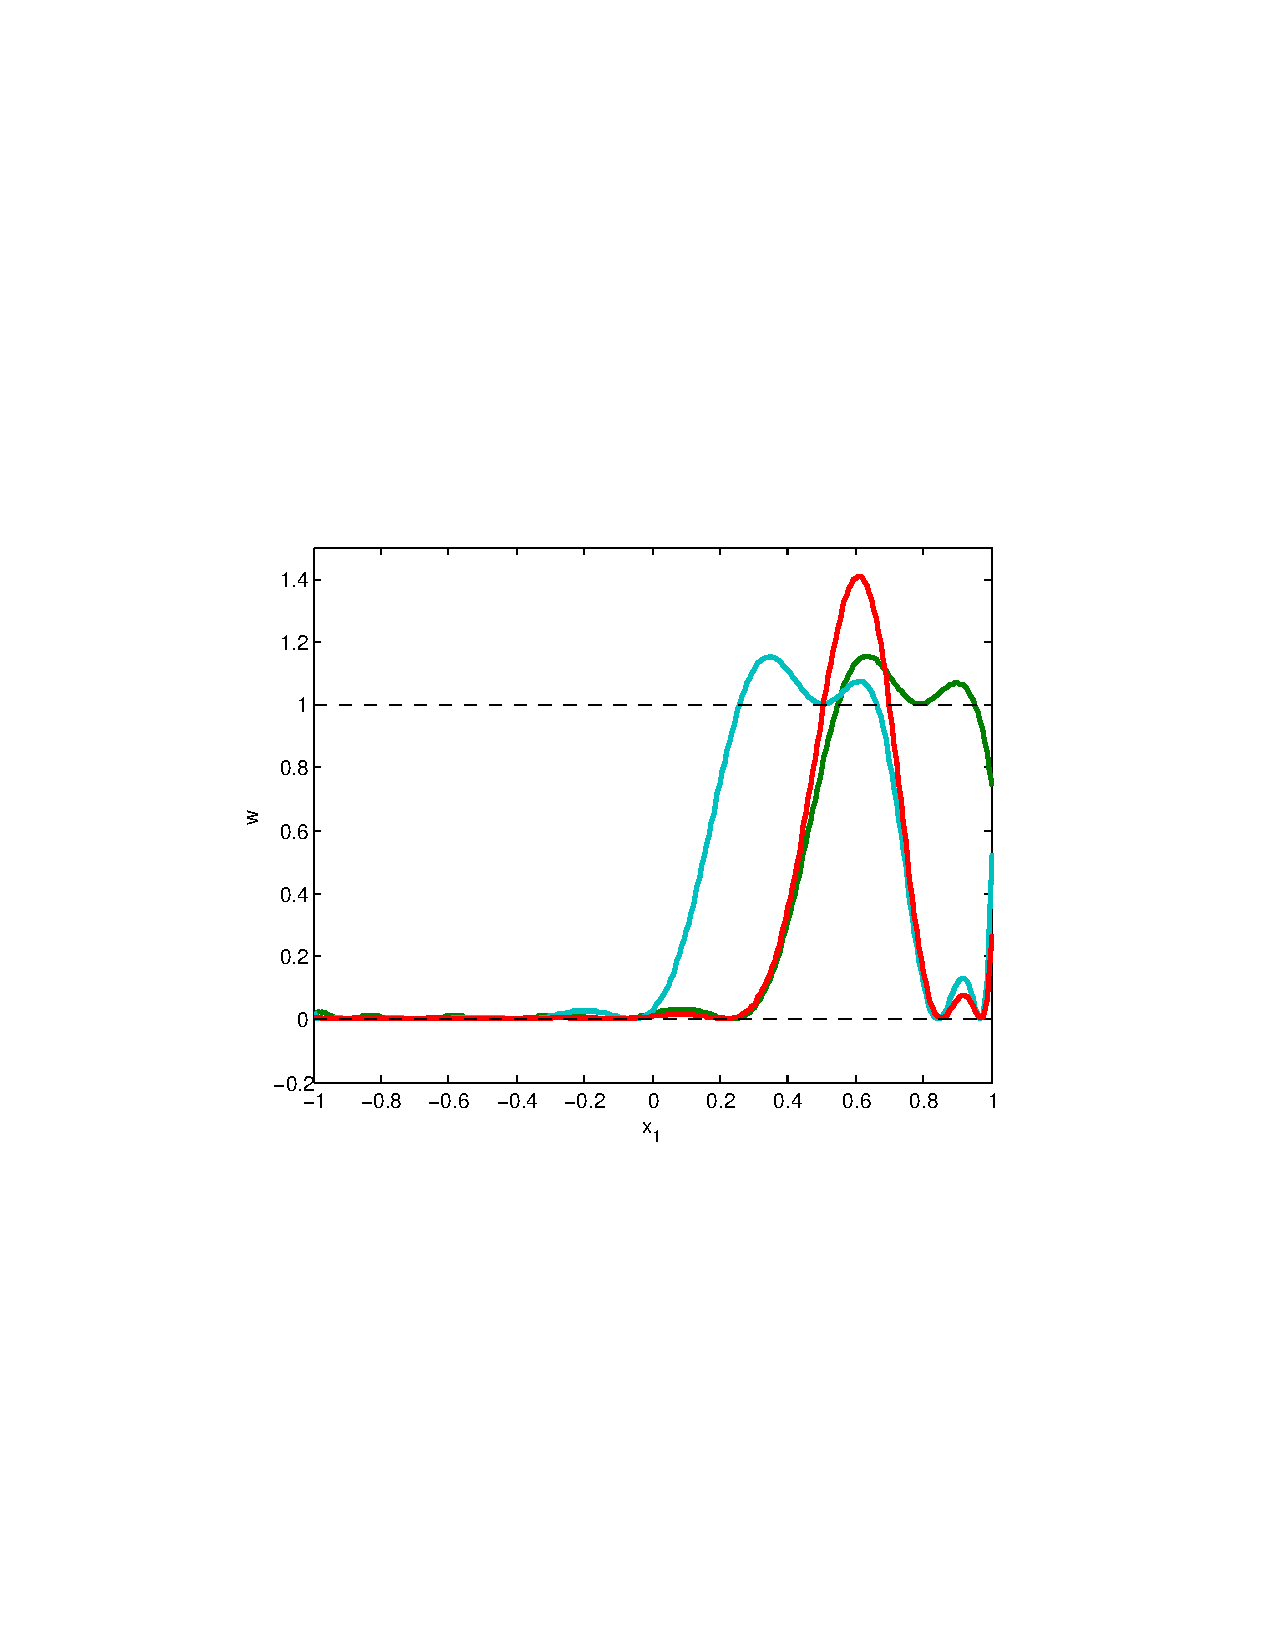
\includegraphics[width=\columnwidth,trim =1.5in 3.3in 1.5in 3.5in, clip=true]{figures/1D_3}
  \caption{Outer approximations of the BRS of the extreme deterministic cases and the stochastic case.(green) $\theta=0$, (blue) $\theta=1$ and (red) $\mu_\theta$}
    \label{fig:1D:linear}
\end{figure}
\par
Figure~\ref{fig:1D:linear} presents the graph of $w_1^{12}$ computed for each of the following cases -- (1) $\theta=0$ (green), (2) $\theta=1$ (cyan), and (3) $\theta\in \mathcal U(0,1)$ (red); when the terminal time is $T=1$ and the terminal set is $\mathcal X_T=[0.2,0.4]$. Observe that the BRS corresponding to case (3) encloses the intersection of those of cases (1) and (2); this is the desired outcome.
\subsection{Rimless wheel}
The planar rimless wheel---constituted by a massless axle to which $n$ equidistant (angular) spokes are connected---is one of the simplest models of legged locomotion. Figure~\ref{fig:rw_schematic} presents a schematic of a rimless wheel---with spokes separated by an angle $2\alpha$---rolling down an infinite wedge. The dynamics of this rimless wheel between transitions is described by
$$
  \begin{bmatrix}
    \dot \theta& \ddot\theta
  \end{bmatrix}'=\begin{bmatrix}
    \dot\theta&\sin(\theta)
  \end{bmatrix}',
$$
where $\theta$ is the angle between the pivoted spoke and the vertical. Once the marching spoke makes contact with the terrain, the states are reset using the maps
$$
  \begin{bmatrix}
    \theta^+&&
    \dot \theta^+
  \end{bmatrix}'=\begin{bmatrix}
    2\gamma-\theta^-&
    \cos(2\alpha)\,\dot\theta^-
  \end{bmatrix}'.
$$
\begin{figure}[!t]
\centering
  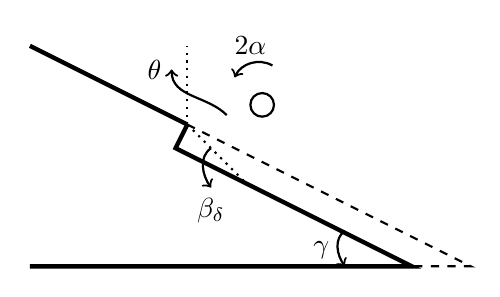
\begin{tikzpicture}
    \draw[-,ultra thick] (0,2) to (2,1);
    \draw[dashed, thick] (2,1) -- (5.6,-0.8)-- (4.85,-.8);
    \draw[ultra thick] (2,1) to (1.85,0.7) -- (4.85,-0.8)--(0,-0.8);
    \draw[thick] (2.95,1.25) circle (.15cm);
    \spoke{(2.95,1.25)}{-75};
    \spoke{(2.95,1.25)}{-15};
    \spoke{(2.95,1.25)}{45};
    \spoke{(2.95,1.25)}{105};
    \spoke{(2.95,1.25)}{165};
    \spoke{(2.95,1.25)}{-135};
    \draw[dotted,thick] (2,1) -- (2,2);
    \draw[dotted, thick] (2,1) -- (2.75,.25);
    \draw[->,thick] (2.3, 0.7) to [out=-145, in =125] (2.3,0.2) node[below] {$\beta_\delta$};
    \draw[->,thick] (4,-.35) to  [out=-145, in =125] (4,-0.8);
    \node at (3.7,-0.6) {$\gamma$};
    \draw[->, thick] (3.08,1.75) to [out=150, in =65] (2.6,1.6);
    \node at (2.8,2) {$2\alpha$};
    \draw[->,thick] (2.5,1.12) to [out=135, in =-90] (1.8,1.7) node[left]{$\theta$};
  \end{tikzpicture}
  \caption{Schematic of the rimless wheel with $\beta_\delta$ being the disturbance.}
  \label{fig:rw_schematic}
\end{figure}
In this example, it is assumed that the slope (terrain) is not flat and that the relative depth of the next step is $\delta$; this translates to an angle $\beta_\delta$ relative to the slope of the wedge. The disturbance to the dynamics of the rimless wheel, $\beta_\delta$, manifests itself in the guard of the only mode in this hybrid system. The angle at which the marching spoke lands on the surface satisfies
$$
  \theta=\gamma+\alpha+\beta_\delta.
$$
An analytically computable stable limit cycle for the disturbance-free rimless wheel exits []; however, for the case considered in this example, the definition of a limit cycle less clear. Consequently, a notion of {\em meta-stability}---when the system states arrive within $\epsilon$ of the stable limit cycle of the disturbance-free system---is adopted.
\par
Figure~\ref{fig:rw_brs} presents the degree 12 BRS (black dashed) for the rimless wheel (with $\alpha=0.4$) which is tasked with arriving within the red band in $T=4$ seconds, as it is rolling down a wedge with slope $\gamma=0.2$ withstanding an a sequence of random changes to terrain drawn from $\beta_\delta\sim\mathcal U([-0.1,0.1])$. The relative depths/height of the disturbance is about 25\% the length of each spoke.
\par
The BRS is validated by performing Monte Carlo simulations; the box $I^2$ is discretized into 51 points both ways and 100 independent trajectories are simulated (using MATLAB's ode45 function) from each initial condition. The blue $\times$s depict the initial conditions that arrived within the terminal set at the desired time without violating any of the other constraints. Note that the set of points that succeeded in the MC simulation is entirely contained in the BRS.
\begin{figure}[!t]
  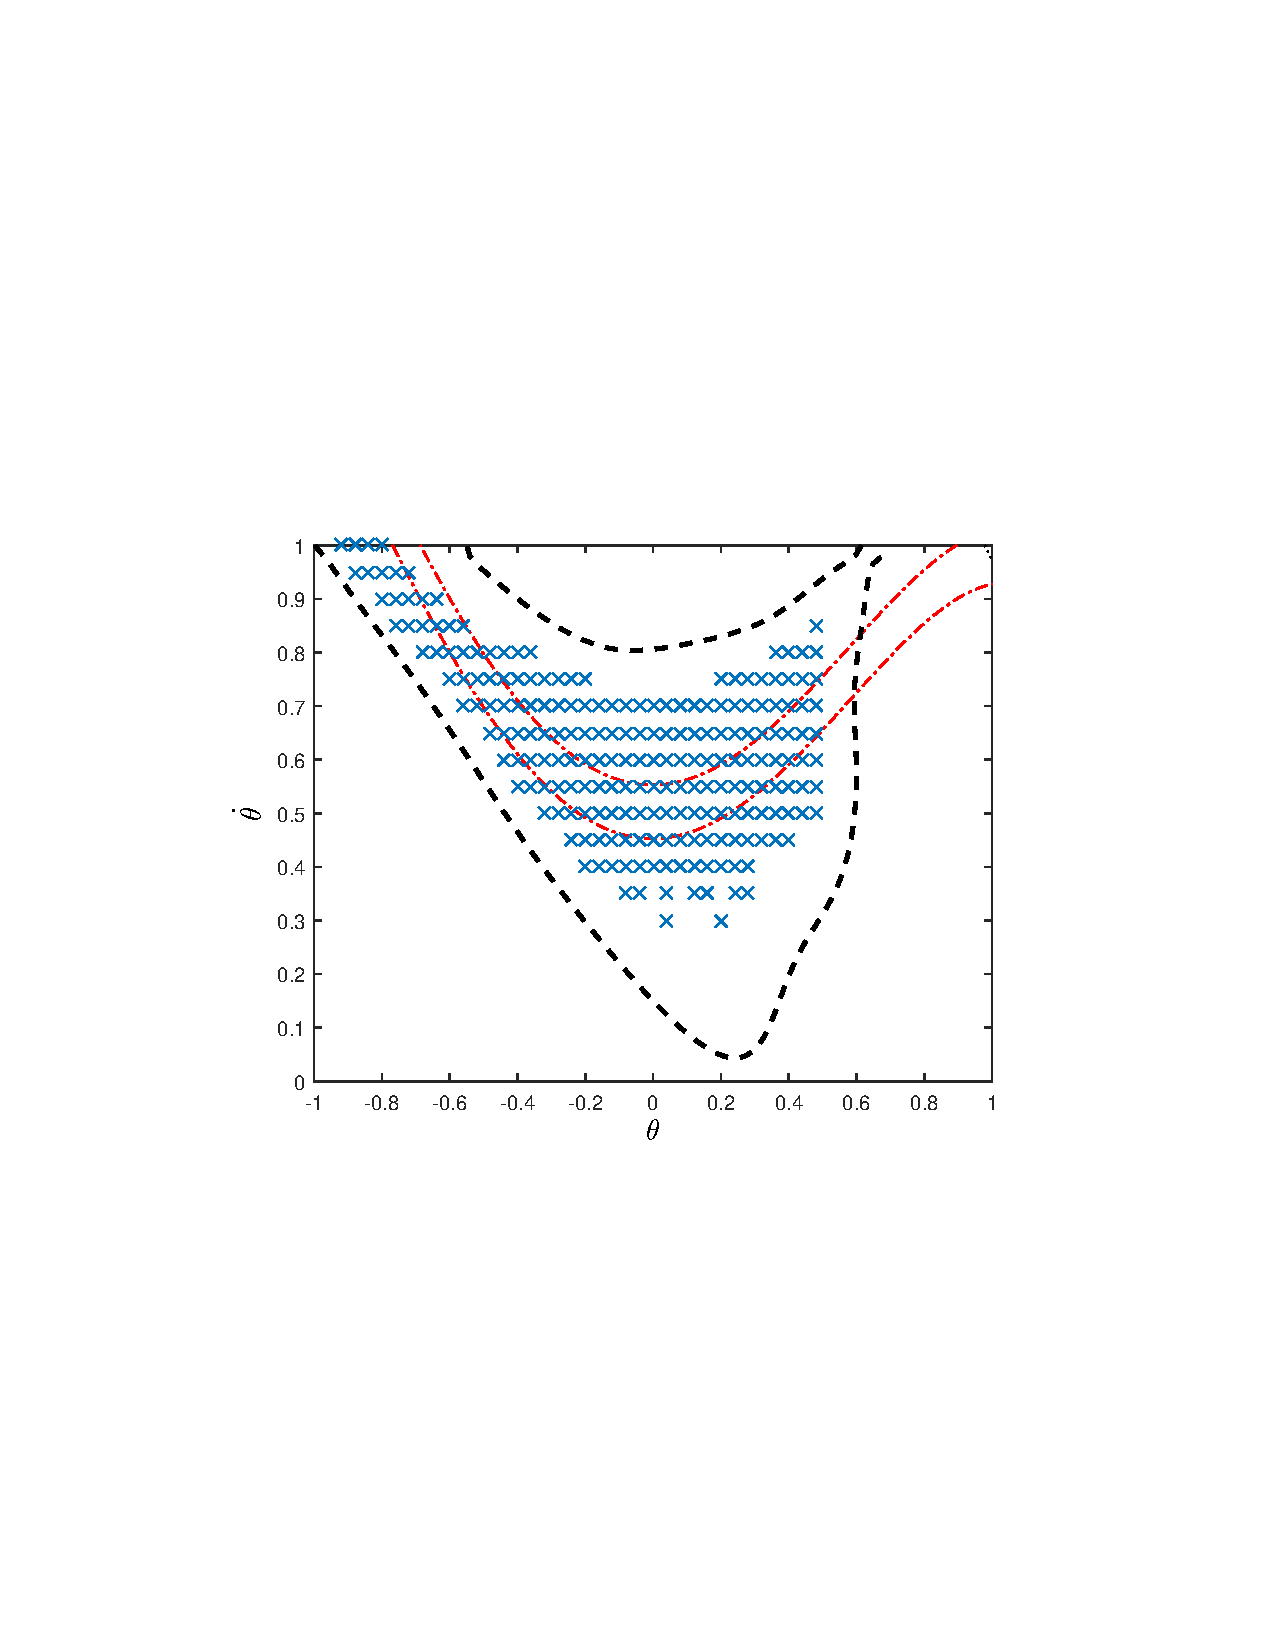
\includegraphics[trim=1.5in 3.3in 1.5in 3.5in, clip=true,width=\columnwidth]{figures/rw_0p1_4}
  \caption{Outer approximation and estimated BRS based on 100 iterations and T=4. Red band is the terminal set and the black outer is the boundary of the estimated BRS; the crosses correspond to results of MC simulation.}
  \label{fig:rw_brs}
\end{figure}
\par
At this juncture, a remark about the tightness of the BRS is warranted. Clearly, the BRS in Fig.~\ref{fig:rw_brs} is not tight; and we attribute this to the set of basis functions with which are currently working--monomials; and the degree relaxation. As commented in [], adopting an alternate basis set is likely to increase the rate of convergence and the tightness. As it stands, there are alternate ways to improve the tightness, primary amongst which is to create phantom modes using identity reset maps; this approach however, needs some care and is deferred for a future work.
